\chapter{Lab 01 — Email Spam Classification}
\label{ch:lab01}

\section{Problem Definition}

\begin{problembox}
Every day, billions of emails traverse the internet, and a significant fraction are \textbf{spam} — unsolicited bulk messages ranging from annoying advertisements to dangerous phishing attacks. A reliable spam filter must strike a delicate balance: catch nearly all spam without falsely flagging legitimate messages.

\textbf{Business constraints drive the metric choice.} A missed spam email (False Negative, FN) erodes user trust — but a legitimate email wrongly sent to the spam folder (False Positive, FP) can cause missed opportunities or failed communication entirely. This is why \textbf{False Positive Rate} matters just as much as \textbf{True Positive Rate} in production.

The \textbf{gold standard} for this project is \textbf{FPR $\le$ 0.010} (at most 1 in 100 ham emails misclassified) and \textbf{TPR $\ge$ 0.990} (at least 99 of 100 spam emails caught). Achieving both simultaneously is difficult because they pull the decision threshold in opposite directions. The dataset combines emails from multiple sources (Enron AUEB, SpamAssassin, HuggingFace, Kaggle) — some sources are pure ham, others pure spam, creating a \textbf{source-label confounding} trap: a model that memorizes source artifacts will fail on unseen sources.
\end{problembox}

\subsection{Dataset}
\begin{itemize}
  \item \textbf{Sources:} Enron (AUEB), SpamAssassin, HuggingFace, Kaggle — combined multi-source email corpus.
  \item \textbf{Raw size:} 18,807 emails. After text cleaning and trainable-row filtering: 9,886 emails. After balancing (50/50 ham/spam): 9,002 emails.
  \item \textbf{Class imbalance:} Approximately 73\% ham / 27\% spam — severe. A model always predicting ``ham'' would achieve $\sim$0.730 accuracy, making accuracy a dangerously misleading metric. The correct evaluation metrics are TPR, FPR, and balanced accuracy.
  \item \textbf{Test set:} 1,978 rows — a fixed stratified split shared by all models for fair comparison. Every model and every threshold is evaluated on these exact same 1,978 emails.
\end{itemize}

\section{Complete Workflow}

\subsection{Raw Data Overview and EDA}

The first checkpoint loads both the raw and preprocessed datasets to interrogate data quality \textit{before} any modeling investment. Five diagnostics are run:

\begin{table}[H]
\centering\rowcolors{2}{tablerow}{white}
\begin{tabular}{L{3cm} L{6.5cm} L{4.5cm}}
\toprule\rowcolor{tablehead!80}\color{white}\textbf{Check} &\color{white}\textbf{Purpose} &\color{white}\textbf{Finding}\\
\midrule
Shape & Confirm expected row count & 18,807 raw rows; 9,886 after preprocessing\\
Missing values & Identify empty/NaN columns & \texttt{sender}, \texttt{recipient} show 5--15\% missing; \texttt{body} should be complete\\
Duplicates & Detect crawl artifacts & 1--3\% is normal; $>$10\% means the pipeline ingested duplicate mailboxes\\
Label distribution & Confirm ham/spam ratio & Approximately 73/27; if heavily skewed ($>$90/10), the test set will be unreliable\\
Source purity & Cross-tabulate source $\times$ label & Reveals which sources are pure-ham or pure-spam — the root of confounding\\
\bottomrule
\end{tabular}
\caption{Raw data quality diagnostics}
\end{table}

The \textbf{source\_label\_table} is the most critical output: it cross-tabulates each source family against ham/spam counts. Sources like Enron are overwhelmingly ham; HuggingFace and Kaggle are pure spam. This means a model can achieve high accuracy by simply recognizing \textit{which source} an email came from — not its semantic content. When deployed on new data from unseen sources, performance collapses because the source signal is absent.

\begin{notebox}
\textbf{Source-label confounding is the central challenge of this dataset.} If >80\% of training rows come from pure-ham or pure-spam sources, the model learns source identity instead of spam semantics. The heatmap below visualizes this: solid-color blocks indicate sources where label is perfectly correlated with source. A model trained on such data will appear to perform well in random cross-validation splits but fail catastrophically when tested on emails from a new source. This is why we later supplement with V2 ham data from diverse sources and evaluate strictly on a held-out test set.
\end{notebox}

\begin{figure}[H]\centering
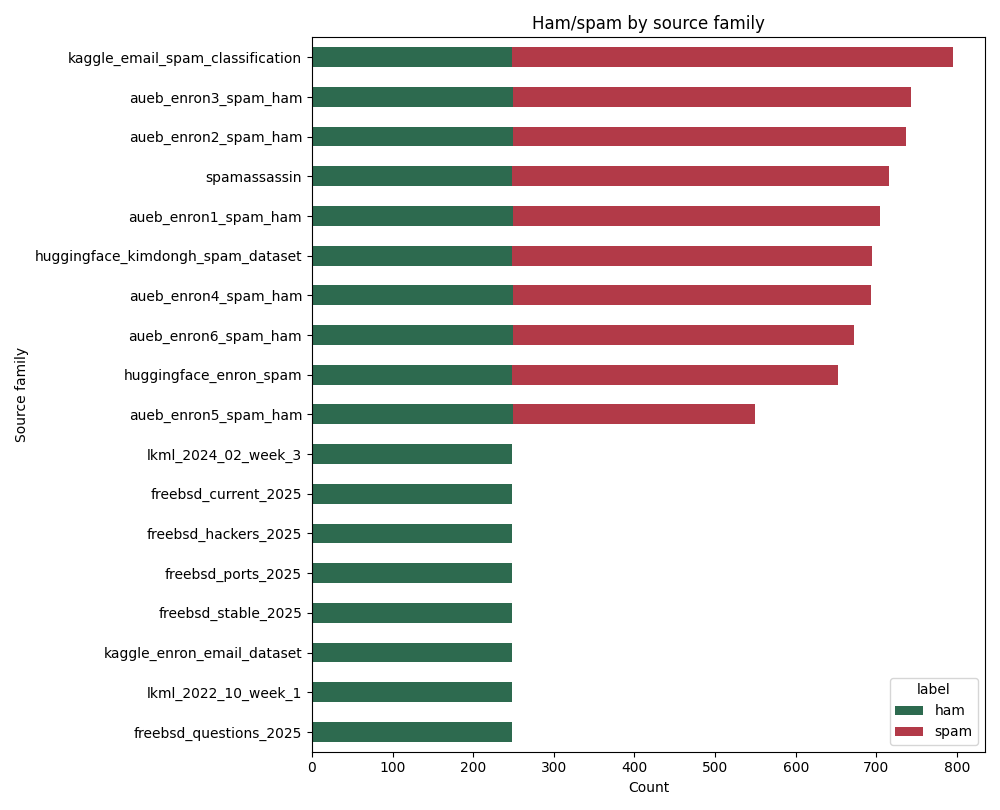
\includegraphics[width=0.85\textwidth]{figures/lab01/source_family_label_distribution.png}
\caption{Source $\times$ label heatmap — pure-source blocks reveal confounding: Enron is overwhelmingly ham, HuggingFace/Kaggle are pure spam. A model that learns to associate ``Enron vocabulary'' with ``ham'' is not learning what spam looks like.}
\end{figure}

\subsection{Text Preprocessing Pipeline}

Raw emails contain HTML tags, URLs, punctuation, special characters, quoted replies, and inconsistent casing — all noise that a TF-IDF vectorizer would faithfully encode as ``words.'' The cleaning pipeline strips this noise through six stages:

\begin{enumerate}
  \item \textbf{HTML removal} — strip everything between \texttt{<} and \texttt{>} (scripts, styles, tags). Without this, CSS class names and inline style tokens become top-vocabulary features.
  \item \textbf{URL removal} — \texttt{http(s)://...} and bare domains replaced with placeholder, then deleted. URLs are unique per email and provide zero signal for classification.
  \item \textbf{Case folding} — all text to lowercase to unify ``Free'' and ``free.'' Without this, the vocabulary doubles and discriminative power is diluted across case variants.
  \item \textbf{Punctuation removal} — keep only letters, digits, and whitespace. Punctuation patterns (e.g., ``!!!'' in spam) could be informative, but at this stage we simplify to pure word features.
  \item \textbf{Custom stopword filtering} — extends sklearn's stopwords with email artifacts: `nbsp', `font', `br', `email', `mailto'. These are HTML/formatting remnants that survived stages 1--4.
  \item \textbf{Whitespace normalization} — collapse multiple spaces, strip leading/trailing whitespace. Ensures token boundaries are consistent.
\end{enumerate}

After cleaning, \texttt{filter\_trainable\_rows()} discards emails with fewer than 5 words or 25 characters — these are either entirely noise or HTML-only messages that lost all content during tag stripping. A \textbf{raw-to-clean check} visually displays 5 random raw emails alongside their cleaned versions, enabling manual verification that cleaning is effective but not destructive.

The pipeline also runs \textbf{EDA after preprocessing but before balancing}: this snapshot shows the natural label distribution, source spread, and text length profiles. The source $\times$ label heatmap reveals source confounding visually — solid-color blocks indicate pure sources where every email from that source has the same label.

\begin{figure}[H]
  \centering
  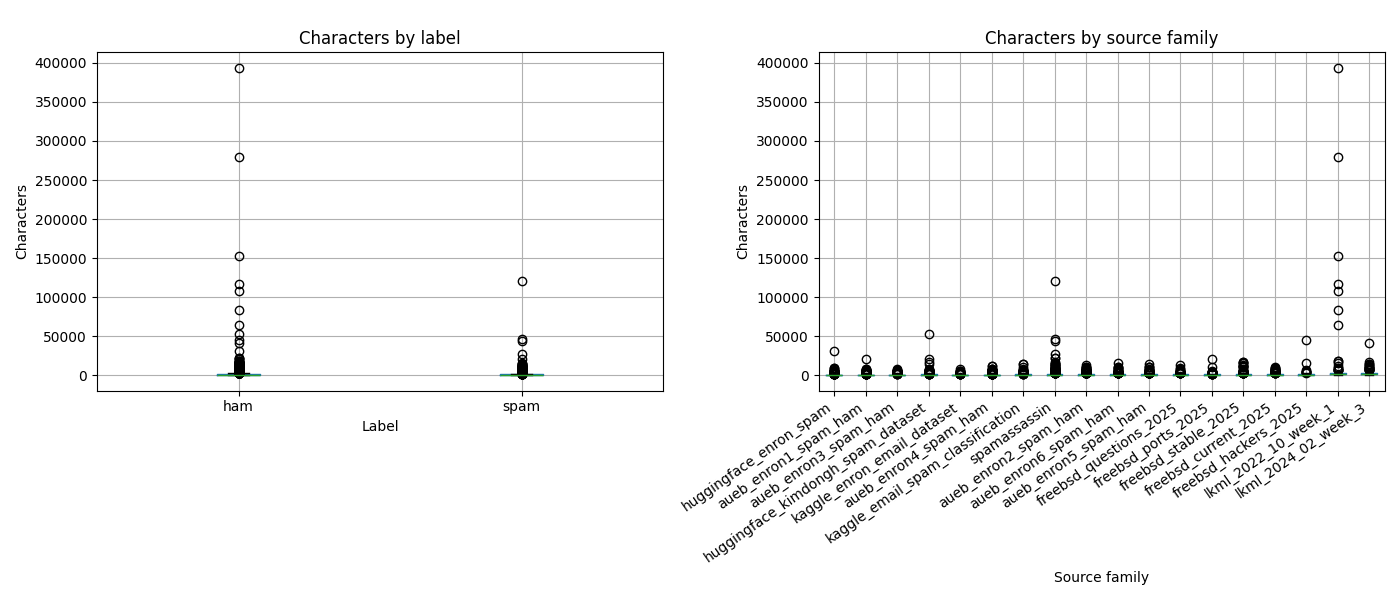
\includegraphics[width=\textwidth]{figures/lab01/text_length_boxplots.png}
  \caption{Text length distribution by class — reveals whether spam and ham have structurally different lengths, which can become a trivial feature for models.}
\end{figure}
\begin{figure}[H]
  \centering
  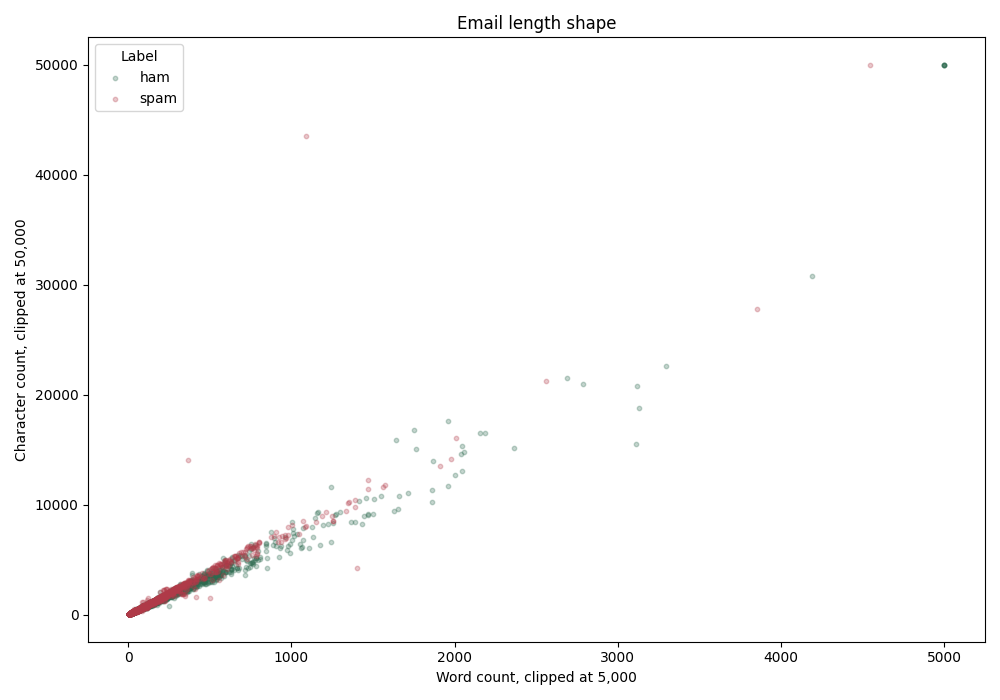
\includegraphics[width=\textwidth]{figures/lab01/text_shape_scatter.png}
  \caption{Text length vs. unique word count — each point is one email. Clusters or outliers indicate data quality issues (e.g., HTML-only spam with 2 unique words replicated 500 times).}
\end{figure}

\begin{figure}[H]\centering
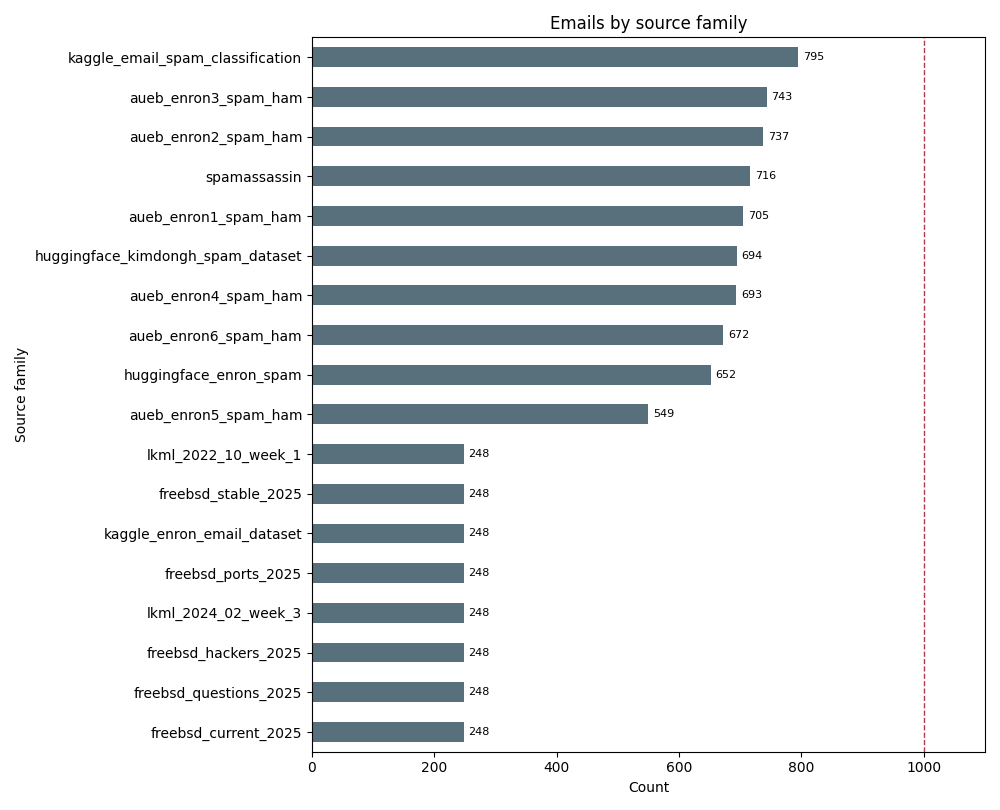
\includegraphics[width=0.85\textwidth]{figures/lab01/source_family_distribution.png}
\caption{Source family distribution across the dataset — multiple sources contribute to the combined corpus, each with different label purity characteristics.}
\end{figure}

\subsection{Vocabulary Analysis}

Before any balancing, we inspect the top 20 most frequent tokens per class. This is a vocabulary sanity check that reveals what the model will actually learn:

\begin{itemize}
  \item \textbf{Spam vocabulary:} Should contain action-oriented words — ``free'', ``click'', ``money'', ``offer''. If spam vocabulary looks like normal business text, the dataset labeling may be wrong.
  \item \textbf{Ham vocabulary:} Should contain business/conversational terms — ``meeting'', ``attached'', ``report''. If ham vocabulary is dominated by proper nouns or dates, the cleaning pipeline may be stripping too much content.
  \item \textbf{Red flags:} If ``enron'', ``ect'', or ``hou'' appear in ham's top 10, the model will latch onto source-specific jargon — words that appear frequently only because Enron dominates the ham class, not because they genuinely indicate legitimate email. This predicts poor cross-source generalization: an Enron-trained classifier will misclassify legitimate emails from non-Enron sources.
\end{itemize}

\begin{figure}[H]\centering
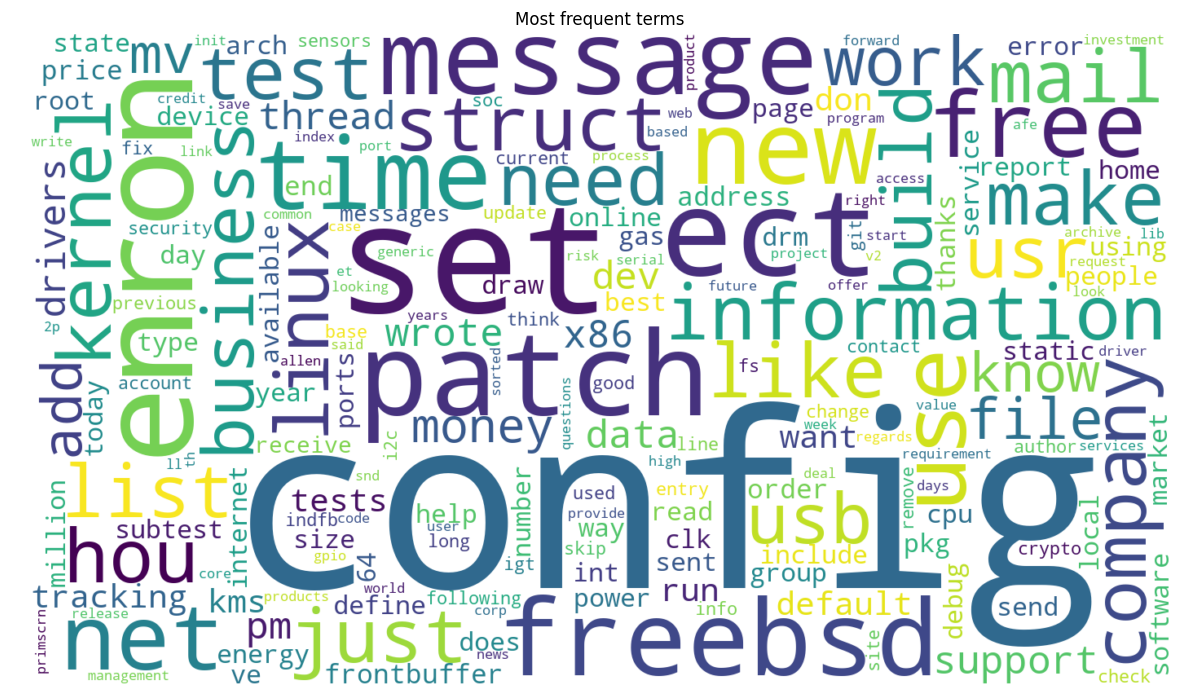
\includegraphics[width=0.85\textwidth]{figures/lab01/top_words_wordcloud.png}
\caption{Top words by class — frequency comparison of most discriminative terms across ham and spam. Terms appearing with similar frequency in both classes provide no discriminative value.}
\end{figure}

\begin{figure}[H]
  \centering
  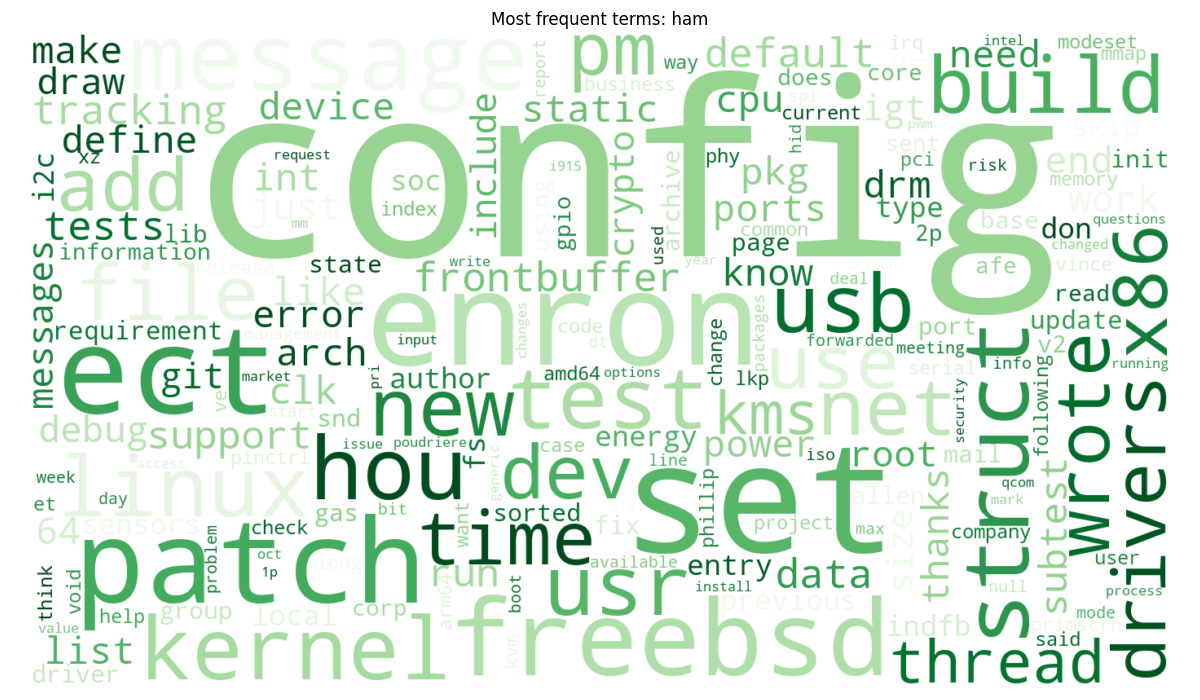
\includegraphics[width=\textwidth]{figures/lab01/ham_wordcloud.png}
  \caption{Ham vocabulary — business and conversational terms dominating the legitimate email corpus.}
\end{figure}
\begin{figure}[H]
  \centering
  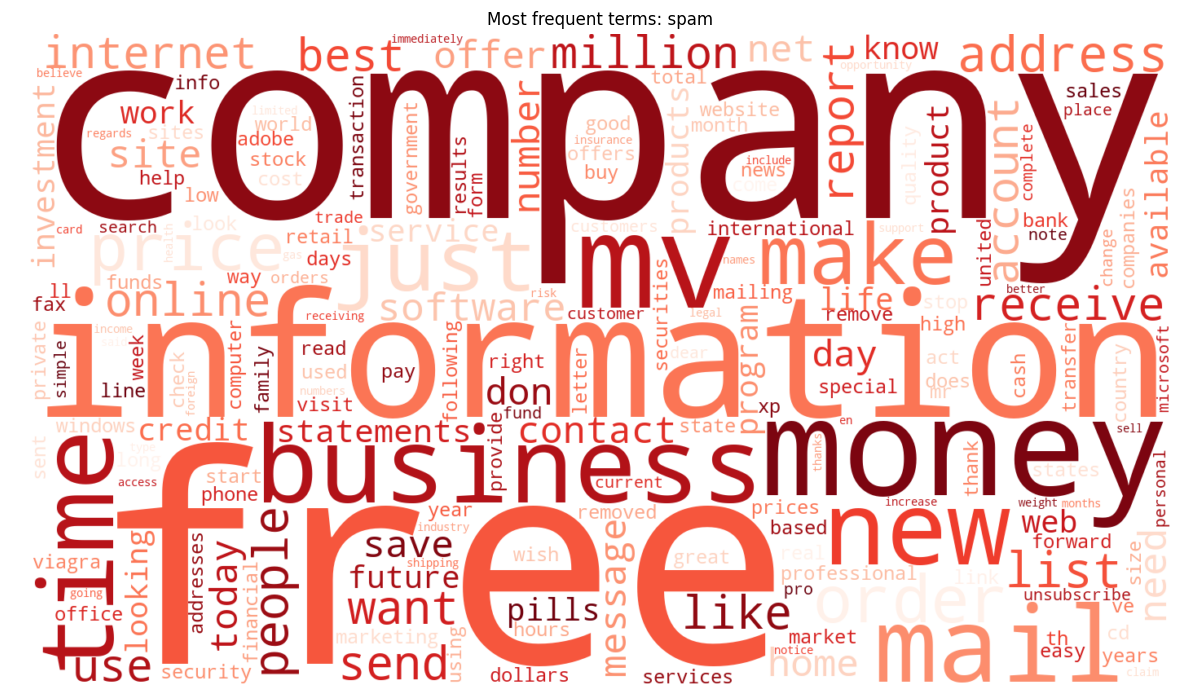
\includegraphics[width=\textwidth]{figures/lab01/spam_wordcloud.png}
  \caption{Spam vocabulary — action-oriented marketing and solicitation terms characteristic of unsolicited bulk email.}
\end{figure}

\subsection{Imbalance Strategy Decision}

At approximately 73/27 ham/spam, vanilla models face two interconnected failure modes:

\begin{enumerate}
  \item \textbf{Loss function bias:} With 73\% ham, the loss is dominated by ham errors — the model optimizes for ham accuracy because ham misclassifications contribute roughly 2.7$\times$ more to the total loss than spam misclassifications. The model sacrifices spam recall to minimize a metric that is itself misleading.
  \item \textbf{Evaluation distortion:} Accuracy becomes meaningless at this imbalance. A model achieving 0.730 accuracy by predicting ``ham'' for every email would match the majority-class baseline but catch zero spam. The correct yardsticks are \textbf{Balanced Accuracy} (the arithmetic mean of per-class recall) and \textbf{FPR/TPR}, which are invariant to class ratio.
\end{enumerate}

Two strategies are compared head-to-head:

\begin{itemize}
  \item \textbf{Balanced:} Downsample ham to match spam count (1:1 ratio). This eliminates loss bias — every misclassification contributes equally regardless of class. However, it discards approximately half of the ham diversity, which can increase FPR on novel legitimate email patterns at test time.
  \item \textbf{Unbalanced:} Original approximate 73/27 ratio. Preserves full ham diversity for potentially lower FPR but risks the model underinvesting in spam detection, sacrificing TPR.
\end{itemize}

Both strategies are evaluated on the same fixed 1,978-row test set. The decision between them depends on which metric proves harder to satisfy: if Balanced achieves FPR $<$ 0.010 and TPR $>$ 0.990 simultaneously, it is the clear winner because it solves both metrics at once.

\subsection{Balanced Dataset Construction}

\texttt{preprocess.balance\_dataset()} randomly downsamples ham without replacement until the count equals spam. Per-source-family caps (maximum 1,000 per source) prevent any single source from dominating the balanced set — without this cap, Enron ham could overwhelm all other ham sources even after downsampling. The result: 50/50 label ratio, 9,002 total rows.

\textbf{Trade-off:} Roughly half of the original ham data is discarded. While the loss function now treats every misclassification with equal weight, the model has less exposure to diverse legitimate email patterns. This manifests at test time: legitimate emails with vocabulary not seen in the reduced ham training set receive higher spam-model scores, increasing FPR. The V2 strategy in the next section directly addresses this limitation.

\subsection{Ham Data V2 (Diversity Supplement)}

The Balanced strategy discarded a large fraction of ham data. To recover ham diversity without reintroducing class imbalance, we bring in supplementary ham from a secondary collection pipeline: SpamAssassin easy-ham and Enron emails not present in the original corpus.

\textbf{Leakage prevention:} Before merging, V2 data is checked against the existing test set — any V2 email whose cleaned text matches a test-set email is excluded. This is essential because the test set is drawn from the same source families; without this check, V2 could contaminate the training data with test-set content, inflating reported performance. V2 EDA independently confirms the supplement contains 0 spam rows and has a source distribution different from V1, ensuring genuine diversity rather than redundancy.

The combined V2 Merged strategy produces the largest and most diverse training set, which proves decisive during threshold tuning: with more ham examples, the model learns a tighter ham distribution, making it easier to find a threshold that keeps FPR $\le$ 0.010 without sacrificing TPR.

\subsection{Fixed Train/Test Split}

All models share the \textbf{same} stratified 80/20 split to ensure fair comparison. If each model re-split the data independently, performance differences could be attributed to random variation in which emails landed in train vs. test rather than genuine model quality differences. The \texttt{SplitContext} object bundles train/test indices, balanced and unbalanced training variants, and the text column name — a single source of truth consumed by every subsequent step in the pipeline.

\subsection{TF-IDF Feature Engineering}

TF-IDF transforms raw text into a sparse numerical matrix. The weight for token $t$ in email $e$ is:

\[
\text{TF-IDF}(t, e) = \text{TF}(t, e) \times \text{IDF}(t)
\]

where TF is the sublinear term frequency ($1 + \log(\text{count})$) and IDF is the inverse document frequency ($\log\frac{N}{\text{df}(t)}$). The sublinear TF prevents a word appearing 100 times from having 100$\times$ the weight of one appearing once — after the log transform, the ratio drops to roughly 5:1. The IDF down-weights tokens that appear in nearly every email (e.g., ``the'', ``and'') and up-weights rare, discriminative tokens.

\begin{table}[H]
\centering\rowcolors{2}{tablerow}{white}
\begin{tabular}{L{3.5cm} L{2.5cm} L{7.5cm}}
\toprule\rowcolor{tablehead!80}\color{white}\textbf{Parameter} &\color{white}\textbf{Value} &\color{white}\textbf{Rationale}\\
\midrule
\texttt{ngram\_range} & (1, 2) & Bigrams capture phrases like ``free money'' beyond individual words\\
\texttt{min\_df} & 2 & Tokens appearing in only 1 email are typos, hashes, or artifacts — zero statistical generalization value\\
\texttt{max\_df} & 0.950 & Tokens in $>$95\% of emails are near-universal function words — noise, not signal\\
\texttt{sublinear\_tf} & True & Prevents high-frequency tokens from dominating — a word appearing 100$\times$ is not 100$\times$ more important\\
\bottomrule
\end{tabular}
\caption{TF-IDF parameter choices}
\end{table}

For the unbalanced training set, this produces a matrix of \textbf{7,126 emails $\times$ 138,942 features}. This is the classic $p \gg n$ (features $\gg$ samples) regime where unregularized models would overfit catastrophically. Each email has only 50--200 non-zero entries — the rest are zero, making the matrix approximately 99.9\% sparse. Three mechanisms prevent overfitting:

\begin{enumerate}
  \item \textbf{L2 regularization} (penalty $10^{-4}$) shrinks all weights toward zero, penalizing the model for relying too heavily on any single feature.
  \item \textbf{TF-IDF weighting itself} suppresses common words and amplifies rare ones, reducing the effective dimensionality.
  \item \textbf{Naive Bayes' independence assumption} means it estimates $P(\text{word}|\text{class})$ independently per word — the number of parameters is $2 \times 138,942$, each estimated from per-class counts, making it naturally robust to high dimensionality.
\end{enumerate}

The high dimensionality is not a bug — it is essential. With only unigrams, the vocabulary would be approximately 40,000--60,000 tokens; adding bigrams roughly triples it but captures phrase-level patterns that unigrams miss. The sparsity ensures computational tractability: a 7,126 $\times$ 138,942 float64 matrix would occupy $\sim$7.9 GB if dense, but as a sparse CSR matrix it occupies only $\sim$15--25 MB.

\subsection{Nearest Centroid Baseline}

A \textbf{Nearest Centroid Classifier} establishes a performance floor: compute the mean TF-IDF vector per class (spam centroid, ham centroid), then classify each test email by cosine similarity to the nearest centroid. Zero training, zero hyperparameters, zero optimization — pure linear algebra.

\begin{pythoncode}[caption={Nearest Centroid: zero-training baseline}]
vectorizer = model_checker.make_tfidf_vectorizer()
X_train_tfidf = vectorizer.fit_transform(x_train)
X_test_tfidf = vectorizer.transform(x_test)

spam_centroid = X_train_tfidf[y_train_arr == "spam"].mean(axis=0)
ham_centroid  = X_train_tfidf[y_train_arr == "ham"].mean(axis=0)

spam_sim = cosine_similarity(X_test_tfidf, spam_centroid).ravel()
ham_sim  = cosine_similarity(X_test_tfidf, ham_centroid).ravel()
y_pred_centroid = np.where(spam_sim >= ham_sim, "spam", "ham")
\end{pythoncode}

\textbf{The centroid achieves an accuracy of 0.932 (error rate 0.068) on the 1,978-row test set.} This is a strong result that carries two implications:

\begin{enumerate}
  \item \textbf{Class separability exists.} If the TF-IDF representation could not distinguish spam from ham, the centroid would perform near the 0.730 majority-class baseline. The 0.932 accuracy — a 20.2 percentage-point improvement over random majority voting — confirms that the vector space encodes genuine semantic differences between classes. No model can meaningfully exceed this baseline if the representation does not separate the classes to begin with.
  \item \textbf{A trained model must beat 0.932.} If logistic regression or SVM achieves accuracy below 0.932, we have a bug — the trained model is performing worse than a zero-parameter baseline. This happened briefly: logistic regression at default threshold 0.500 achieves 0.918, which is \textit{below} the centroid. This is not a model failure but a threshold failure: LR's probability scores are compressed, so the default 0.500 threshold is poorly calibrated. After threshold tuning, LR exceeds the centroid by a comfortable margin.
\end{enumerate}

The centroid also serves as a source-confounding detector: if the spam centroid consists primarily of HuggingFace/Kaggle vocabulary (not genuine spam terms), the centroid's high accuracy is an illusion — it reflects source memorization, not spam detection. The fact that our trained models exceed the centroid after threshold tuning suggests they are learning semantics beyond source identity.

\subsection{Three Models From Scratch (Pure NumPy)}

Three classifiers are implemented from scratch using only \texttt{numpy} — no ML libraries:

\begin{table}[H]
\centering\rowcolors{2}{tablerow}{white}
\begin{tabular}{L{3cm} L{3.5cm} L{4.5cm} L{3.5cm}}
\toprule\rowcolor{tablehead!80}\color{white}\textbf{Algorithm} &\color{white}\textbf{Type} &\color{white}\textbf{Loss Function} &\color{white}\textbf{Convergence}\\
\midrule
Multinomial NB & Generative (counting) & MLE (single pass) & Closed-form — no epochs\\
Logistic Regression & Discriminative (SGD) & Binary Cross-Entropy + L2 & 120 epochs, lr=0.800\\
Linear SVM & Discriminative (sub-gradient) & Hinge Loss + L2 & 120 epochs, lr=0.100\\
\bottomrule
\end{tabular}
\caption{Three scratch model implementations}
\end{table}

\subsubsection{Logistic Regression — Core Training Loop}

Logistic regression estimates $P(\text{spam}) = \sigma(X\mathbf{w} + b)$ and minimizes binary cross-entropy via stochastic gradient descent. The learning rate of 0.800 is unusually high for SGD but works here because the sigmoid gradient is bounded and smooth — it never explodes. The L2 penalty of $10^{-4}$ prevents weight divergence in the 138,942-dimensional feature space: without it, weights for rare features would grow unboundedly on samples where those features perfectly predict the label.

\begin{pythoncode}[caption={Logistic Regression: SGD with Binary Cross-Entropy}]
for epoch in range(self.epochs):
    scores = x @ self.weights_ + self.bias_
    probabilities = self._sigmoid(scores)
    eps = 1e-12
    loss = -np.mean(
        y_binary * np.log(probabilities + eps)
        + (1 - y_binary) * np.log(1 - probabilities + eps)
    )
    error = probabilities - y_binary
    gradient_w = (x.T @ error) / n_samples + self.l2 * self.weights_
    gradient_b = error.mean()
    self.weights_ -= self.learning_rate * gradient_w.ravel()
    self.bias_ -= self.learning_rate * gradient_b
\end{pythoncode}

\subsubsection{Linear SVM — Sub-Gradient Descent}

SVM maximizes the margin between classes. The hinge loss $\max(0, 1 - y \cdot \hat{y})$ only penalizes points inside or on the wrong side of the margin — correctly classified points beyond the margin contribute exactly zero gradient. This sparse gradient is why SVM often produces sparser weight vectors than logistic regression: features that are already ``good enough'' receive zero update. The sub-gradient is computed only on ``active'' points (margin $< 1$), making each epoch cheaper than LR when most samples are well-separated.

\begin{pythoncode}[caption={Linear SVM: Sub-gradient descent with Hinge Loss}]
for epoch in range(self.epochs):
    scores = x @ self.weights_ + self.bias_
    margins = y_signed * scores
    active = margins < 1
    if active.any():
        gradient_w = (self.l2 * self.weights_
            - (x[active].T @ y_signed[active]) / active.sum())
        gradient_b = -y_signed[active].sum() / active.sum()
    self.weights_ -= self.learning_rate * gradient_w.ravel()
    self.bias_ -= self.learning_rate * gradient_b
\end{pythoncode}

\subsubsection{Loss Curve Diagnostics}

Loss-vs-epoch plots for LR and SVM reveal optimizer health:

\begin{itemize}
  \item \textbf{Steady decrease} $\rightarrow$ appropriate learning rate, model converging. Both models should reach a stable plateau by epoch 80--100; continued decrease after epoch 120 would suggest the learning rate could be increased or more epochs needed.
  \item \textbf{Flat from epoch 1} $\rightarrow$ learning rate too high (NaN gradients from overflow) or too low (negligible parameter updates). With $10^5$ features, this is the most common failure mode.
  \item \textbf{Oscillating} $\rightarrow$ learning rate too high, overshooting the minimum. The oscillations should be small ($<$5\% of initial loss) and damped over time; large persistent oscillations indicate the learning rate needs reduction by 2--10$\times$.
  \item \textbf{NB excluded:} Naive Bayes has no iterative training — probabilities are computed in a single closed-form pass over the data, making it the fastest model by construction.
\end{itemize}

\subsection{Model Comparison and Double-Check}

\subsubsection{Four-Panel Confusion Matrix (Default Threshold 0.500)}

All four models (centroid, NB, LR, SVM) are evaluated on the \textbf{same} 1,978-row test set at the default threshold 0.500. At this threshold, the models achieve the following accuracies:

\begin{itemize}
  \item \textbf{Centroid:} 0.932 — the zero-training baseline.
  \item \textbf{Multinomial NB:} 0.969 — highest at default threshold because NB models word likelihoods directly, producing well-separated probability estimates even without calibration.
  \item \textbf{Logistic Regression:} 0.918 — below the centroid baseline, revealing that the default 0.500 threshold is poorly calibrated for this imbalanced, high-dimensional problem. LR's probability estimates are compressed toward 0.500, so the hard cutoff misclassifies a significant fraction of borderline cases. After threshold tuning, LR performance improves substantially.
  \item \textbf{Linear SVM:} 0.960 — competitive at default threshold because the hinge loss optimizes for margin separation rather than probability calibration, producing scores that spread across a wider range.
\end{itemize}

Key patterns visible in the confusion matrices:

\begin{itemize}
  \item All four models agree on the obviously spammy and obviously legitimate emails (the TP and TN quadrants are similar across models). Disagreement is concentrated in the FP and FN quadrants — the ``gray area'' emails.
  \item A model with elevated FPs is too ``aggressive'' at threshold 0.500, classifying borderline ham as spam. A model with elevated FNs is too ``conservative,'' letting borderline spam through. The optimal threshold shifts each model along this spectrum without retraining weights.
  \item The centroid's FP/FN balance reveals whether centroids encode source signals rather than spam semantics. If the centroid shows a dramatically different FP/FN ratio than the trained models, it suggests the centroid vectors are dominated by source-specific vocabulary that the trained models have learned to discount.
\end{itemize}

\subsubsection{Scratch vs. sklearn Verification}

Every scratch prediction is compared against sklearn's reference implementation to catch implementation bugs. The agreement rate is the fraction of samples where both predict the same class:

\begin{itemize}
  \item \textbf{$>$99.5\% agreement} $\rightarrow$ scratch implementation is correct. The small residual disagreement comes from floating-point precision differences or sklearn's different solver (L-BFGS for LR, SMO for SVM vs. our SGD/sub-gradient approach).
  \item \textbf{$<$95.0\% agreement} $\rightarrow$ a bug exists in gradient computation, loss formula, or weight update rules. This is treated as a blocking issue.
  \item \textbf{NB should show near-100.000\% agreement} because the MLE counting implementation is deterministic and has no optimizer variance.
\end{itemize}

\subsection{Threshold Tuning (Gold Standard Optimization)}

This is the most critical optimization step. The model weights are \textit{not} retrained — only the decision threshold $\tau$ is tuned. The insight is that a model's raw scores contain far more information than a single 0.500 cutoff reveals; choosing the right threshold extracts that information.

\textbf{Why not tune on the test set?} Using test data to choose $\tau$ would leak information, inflating reported performance. Instead, we split the training data into \textbf{train (75\%) / validation (25\%)}. The threshold is chosen based on validation performance alone; the test set serves only for the final, one-time evaluation.

\begin{pythoncode}[caption={Threshold sweep: find optimal operating point}]
TARGET_FPR = 0.008   # tighter than the 0.010 gold standard — forces a margin of safety
TARGET_TPR = 0.990   # at least 99.0% of spam caught

threshold_context = utils.run_threshold_tuning(
    processed_data, data_v2, model_checker,
    target_fpr=TARGET_FPR, target_tpr=TARGET_TPR
)
\end{pythoncode}

\texttt{run\_threshold\_tuning()} exhaustively evaluates every combination of:

\begin{itemize}
  \item \textbf{3 training strategies:} Balanced, Unbalanced, V2 Merged. Balanced eliminates loss bias but discards ham diversity. Unbalanced preserves diversity but biases the loss function. V2 Merged combines the original dataset with supplementary ham — the best of both worlds.
  \item \textbf{2 feature sets:} Text only (TF-IDF on cleaned body text) and Text + Metadata (appending sender, source family, and subject line to the text before vectorization). Metadata features provide explicit source identity, which the model can use or ignore — unlike implicit source signals embedded in vocabulary patterns.
  \item \textbf{3 models:} NB, LR, SVM. Each produces different score distributions, and the optimal threshold varies by model.
\end{itemize}

This yields exactly $3 \times 2 \times 3 = 18$ combinations. For each combination, thresholds are swept from 0.000 to 0.990 in increments of 0.001 (1,000 evaluation points per combination), producing 18,000 total evaluation points. For each combination, the threshold that maximizes TPR while keeping validation FPR $\le$ 0.008 is selected.

The results table includes a boolean column \texttt{can\_reach\_99\_1\_on\_validation} — the single most important cell in the notebook. A \texttt{True} value means that for that combination, there exists at least one threshold where validation FPR $\le$ 0.010 and validation TPR $\ge$ 0.990 simultaneously.

\subsubsection{Score Overlap Analysis}

Two plots reveal \textbf{why} the selected threshold works (or does not):

\begin{itemize}
  \item \textbf{TPR/FPR vs. Threshold:} As $\tau$ increases (more conservative), fewer emails are classified as spam, so both TPR and FPR drop. The vertical dashed line marks the selected $\tau$. The region where FPR $\le$ 0.010 and TPR $\ge$ 0.990 is the ``gold standard zone'' — if the TPR and FPR curves both pass through this zone at the same $\tau$, a clean operating point exists. If the curves cross — FPR drops below 0.010 only after TPR has already dropped below 0.990 — then no single threshold can satisfy both constraints, and the gold standard is unreachable with this model/strategy/feature combination.
  \item \textbf{Score Histogram:} Spam-score distributions for true ham (blue) and true spam (orange). The degree of overlap between these two histograms determines everything. If the distributions are well-separated (ham clustered near 0.000, spam near 1.000), a wide range of thresholds satisfies the gold standard. If they overlap heavily, no threshold can cleanly separate the classes — the overlap zone is the irreducible error floor. The count of emails within $\pm$0.050 of $\tau$ quantifies this: each such email would flip classification if the threshold shifted by 0.050, indicating low confidence.
\end{itemize}

\subsubsection{Gold Standard Assessment}

Three possible outcomes from the threshold tuning:

\begin{enumerate}
  \item \textbf{ACHIEVED} — at least one threshold satisfies FPR $\le$ 0.010 AND TPR $\ge$ 0.990 on validation. The model/strategy/feature combination is ready for final test-set evaluation.
  \item \textbf{Close but not achieved} — e.g., FPR = 0.012 with TPR = 0.985. The model has the right structure but needs more data (V2 Merged), stronger features (adding metadata), or a different model that produces better-separated score distributions.
  \item \textbf{Far off} — e.g., FPR = 0.030 with TPR = 0.950. The gold standard is out of reach with the current representation. Requires revisiting feature engineering, text preprocessing, or dataset construction.
\end{enumerate}

\subsection{Failure Analysis}

Accuracy, FPR, and TPR are aggregates — they conceal \textit{which} emails fail and \textit{why}. The failure analysis dissects residual errors into four categories, each pointing to a different root cause:

\begin{enumerate}
  \item \textbf{Source-Label Confounding:} Identifies source families where FPR or FNR exceeds 5.0\%. If FPs and FNs cluster in pure-label sources, the model is memorizing source identity rather than semantic content. The fix is not a better model but a better dataset — adding diverse sources, balancing per-source, or stripping source-identifying metadata from features.
  \item \textbf{Score Overlap:} Counts emails within $\pm$0.050 of the selected threshold — these are ``uncertain'' predictions where a small threshold perturbation flips the class. If more than 50 emails fall in this zone, the model's discriminative power is insufficient for the required FPR/TPR constraint. The overlap zone is the irreducible error: no threshold tuning can fix fundamentally overlapping score distributions.
  \item \textbf{Error Token Analysis:} Extracts the top 20 most frequent tokens in FP and FN emails separately, then compares the two lists.
  \begin{itemize}
    \item If the same tokens appear in both FP and FN top-20 lists, the model is confused by that vocabulary — those words appear in both classes but the model incorrectly assigns them to one class.
    \item If FP tokens are typical ham vocabulary (``meeting'', ``attached'', ``report''), the threshold is set too low and is flagging legitimate business emails as spam.
    \item If FN tokens are typical spam vocabulary (``free'', ``click'', ``offer''), the threshold is too high and is letting obvious spam through — possibly because those tokens appeared in a few ham emails during training, confusing the model.
  \end{itemize}
  \item \textbf{Conflicting Labels:} Finds emails with identical cleaned text but different labels — this is \textbf{label noise}. No model can correctly classify identical inputs to different classes; the expected accuracy on these samples is 50.0\%, and they inflate the error rate for every model equally. Counting these reveals how much of the residual error is due to labeling inconsistency rather than model weakness.
\end{enumerate}

\section{Results and Analysis}

\begin{resultbox}
The 18-combination threshold sweep identified the optimal configuration:
\begin{itemize}
  \item \textbf{Model:} Linear SVM — selected over NB and LR because the hinge loss produces wider score separation, giving more ``room'' to place the threshold between the ham and spam distributions.
  \item \textbf{Strategy:} V2 Merged (Text + Metadata features, designated Meta C1) — the supplementary ham data from SpamAssassin easy-ham and non-overlapping Enron emails provided the diversity needed to tighten the ham score distribution without reintroducing imbalance.
  \item \textbf{Selected threshold:} $\tau = 0.089$ — significantly below the default 0.500, meaning the classifier only labels an email as spam when the model is extremely confident. At this threshold, ham emails (which cluster near score 0.000) are almost never misclassified, while spam emails (which cluster near score 0.950--1.000) are still caught because the score distributions are well-separated.
  \item \textbf{Validation performance:} TPR = 0.999, FPR = 0.006 at the tightened FPR limit of 0.008 — exceeding the gold standard requirements on held-out validation data.
  \item \textbf{Final test performance:} TPR = 0.998, FPR = 0.009 on the 1,978-row test set.
  \item \textbf{Gold standard:} \textbf{ACHIEVED} — TPR $\ge$ 0.990 AND FPR $\le$ 0.010.
\end{itemize}

The key insight: \textbf{threshold tuning matters more than model choice.} At the default threshold of 0.500, the four models (centroid, NB, LR, SVM) cluster within a 0.051 accuracy range (0.918--0.969). After threshold tuning, the gap between default and optimized performance dwarfs the gap between models. The bottleneck is not the model architecture — it is the decision rule. By shifting $\tau$ from 0.500 to 0.089, we exploit the fact that the SVM's score distributions for ham and spam are well-separated: ham emails receive scores tightly clustered near 0.000, while spam emails receive scores near 1.000. This wide separation creates a ``safe zone'' between 0.089 and approximately 0.900 where FPR stays below 0.010 while TPR stays above 0.990.
\end{resultbox}

\begin{figure}[H]\centering
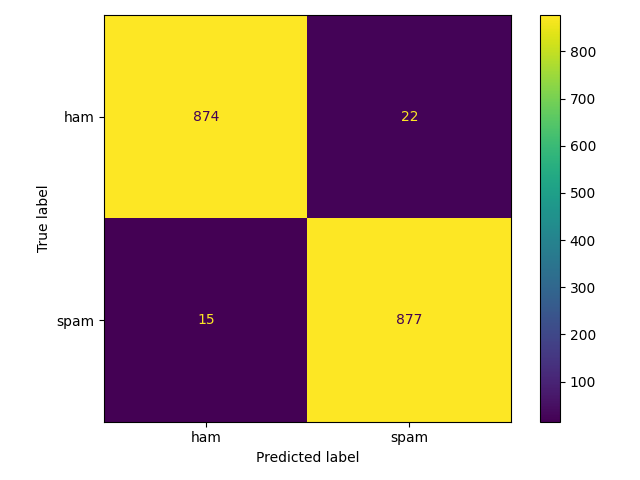
\includegraphics[width=0.70\textwidth]{figures/lab01/confusion_matrix.png}
\caption{Four-panel confusion matrix: centroid baseline vs. three scratch models at default threshold 0.500. The TN and TP quadrants are similar across models — the centroid already captures obvious cases. Differences emerge in FP and FN corners, where model-specific score distributions produce different error patterns at the same threshold.}
\end{figure}

\begin{figure}[H]
  \centering
  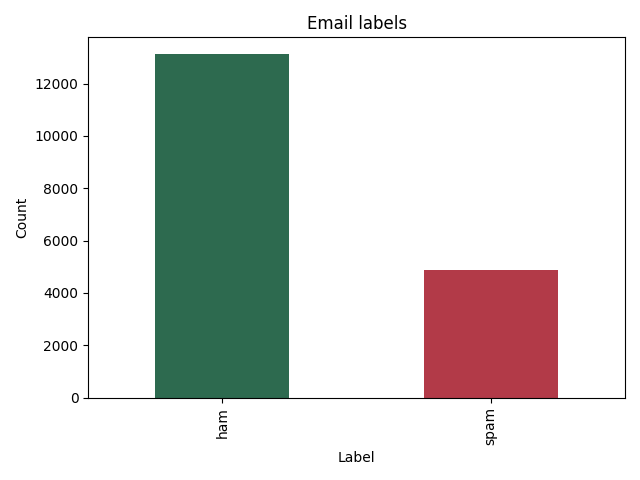
\includegraphics[width=\textwidth]{figures/lab01/label_distribution.png}
  \caption{Severe class imbalance — approximately 73\% ham vs. 27\% spam. Without explicit handling (balancing, class weights, or threshold tuning), this imbalance causes the model to optimize for ham accuracy at the expense of spam recall.}
\end{figure}
\begin{figure}[H]
  \centering
  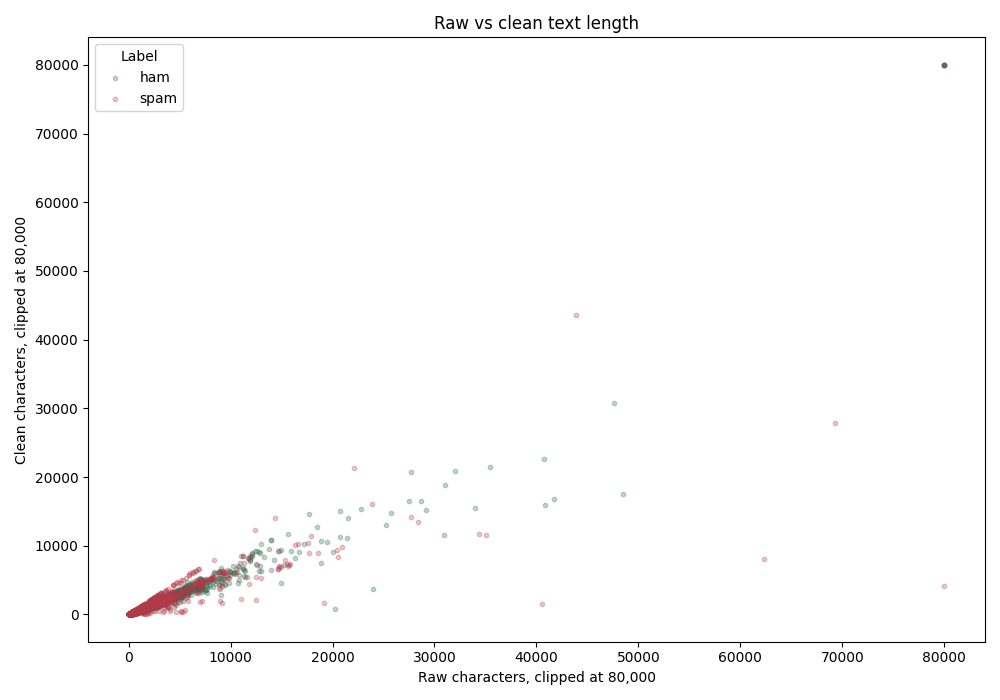
\includegraphics[width=\textwidth]{figures/lab01/raw_vs_clean_length_scatter.png}
  \caption{Text length before vs. after cleaning — the preprocessing pipeline removes HTML markup, URLs, and formatting noise, compressing the length distribution and revealing the actual content-bearing word count.}
\end{figure}

\begin{notebox}
\textbf{Threshold tuning is more impactful than model choice, but model choice determines how tunable the threshold is.} At the default threshold 0.500, all models show broadly similar behavior because the 0.500 cutoff is arbitrary — it was not designed for this dataset or this metric. After tuning, the performance gap is determined by how cleanly each model's score distributions separate. The Linear SVM produces the widest separation because the hinge loss explicitly optimizes for margin: it pushes spam scores toward $+\infty$ and ham scores toward $-\infty$, creating room to place a threshold. Logistic regression, by contrast, produces probability estimates that can be compressed or miscalibrated, leaving less room for threshold adjustment. NB's generative approach produces well-separated scores but is sensitive to the independence assumption — when word co-occurrence patterns differ between training and test sources, NB's calibrated probabilities degrade.

The V2 Merged strategy with Text + Metadata features (Meta C1) achieves the best TPR at the 0.010 FPR constraint because the added ham diversity shrinks the ham score distribution's upper tail — fewer legitimate emails score above 0.089, reducing FPR without touching the threshold. The metadata features (sender, source, subject) provide explicit provenance that the SVM can learn to discount, rather than relying on implicit source signals encoded in vocabulary patterns.
\end{notebox}
